% ********** Testbeds Chapter **********
\chapter{Cryogenic Testbeds}
\label{cha:testbeds}
%
\section{Introduction}\label{sec:testbeds_Introduction}
As is the case with all ultra-sensitive mid- to far-infrared detectors \parencite[as described by][]{Richards1994}, the silicon cold electron bolometer requires cooling to extremely low temperatures in order to operate. This requirement can be seen from the description of cold electron bolometers given in Chapter~\ref{cha:theory}. Since these detectors incorporate superconducting contacts to select only the most energetic (i.e. the hottest) electrons from the detector's absorber, it is important that the superconductor is cooled sufficiently that the superconducting energy gap is close to its maximum. For the detectors studied in this work, which used aluminium contacts, it was found \reminder{Add cross-ref} that cooling to approximately $\sim \nicefrac{T_{c}\,}{4}$ ($300~\mathrm{mK}$) allowed the detector to operate reasonably. However, in order to arrive at as complete a study as possibly it was important to measure the electrical properties of the detectors to as low a temperature as possible.
\par 
To this end several different cryogenic systems have been used in the course of this work. The most significant of these (those in which results presented in this thesis were taken) were: an \glsfirst{gls:ADR} housed in a liquid helium cryostat, a He10 sorption refrigerator housed in a cryostat with a pulse tube cooler, and a He7 sorption refrigerator mounted on the cold plate of a liquid helium cryostat.\footnote{Note: He7 and He10 here do not denote some strange and exotic isotopes of helium but instead the combination of pumps which make up the soprtion refrigerator. Isotopes have been typeset with a leading superscript (i.e. \ce{^{4}He}). A He7 refrigerator contains one \ce{^{4}He} pump and a \ce{^{3}He} pump, a He10 refrigerator consists of a He7 refrigerator used as a buffer stage for a second \ce{^{3}He} pump.} The reason for the use of these numerous system was essentially due to availability and the associated costs of liquid helium. Primary measurements were carried out in the pulse tube cooled cryostat since this had lower running costs (due to not requiring a reservoir of liquid helium to be maintained). However (as will be seen later in this chapter), the system was not designed with the dc readout of sensitive detectors in mind and resulted in lower quality data than would have been desired; however it did provide a useful facility for asserting whether or not a device was functional. The two other systems, both of which required the supply of liquid helium, were used for very specific purposes. The \glstext{acr:ADR} system was used to measure device down to extremely low temperatures (the minimum temperature achieved with this system was $80~\mathrm{mK}$) whereas the system containing a He7 refrigerator contained optical windows, horns and filters to allow the detector to observe external sources. This chapter will cover the operational principles along with the cryogenic performance and suitability for the required measurements of each of these systems.
%
\section{Sorption Refrigerators}\label{sec:sorptionRefrigerators}
Sorption refrigerators operate by the adsorption and desorption of a working gas (helium in the case of systems intended to operate at cryogenic temperatures) from a surface or other material (most commonly activated charcoal). The released gas flows through a pipe until it is cooled by a condensation point and liquified. This liquid is collected in a stage called the evaporator. The activated charcoal is then cooled causing the gas evaporating from the liquid in the evaporator to become reattached to the charcoal thus decreasing the pressure in the system and thus the temperature of the liquid in the evaporator. An artistic impression of a single-stage sorption refrigerator is shown in Figure~\ref{fig:sorptionPumpCrossSec}
\begin{figure}[tb]
\begin{center}
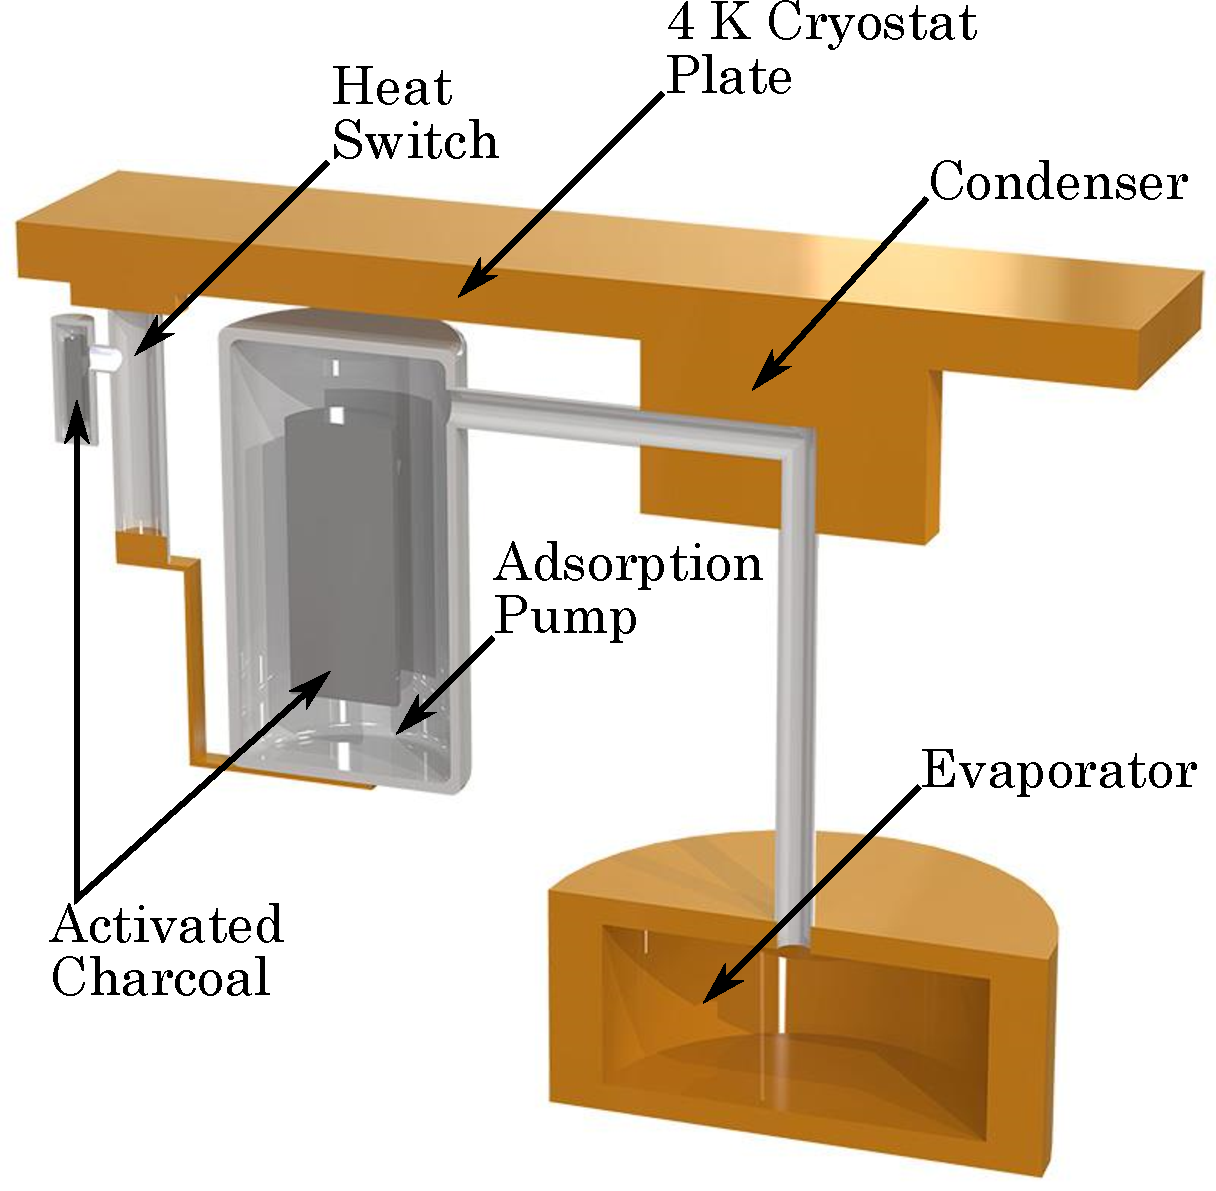
\includegraphics[width = 0.6\textwidth]{figures/sorptionPump.pdf}
\caption[Artistic impression of the cross section of a sorption refrigerator]{Artistic impression of the cross section of a sorption refrigerator. The 4-Kelvin plate of the cryostat is cooled by either a liquid-helium reservoir or a mechanical cooler (not shown in either case).}
\label{fig:sorptionPumpCrossSec}
\end{center}
\end{figure}
\par 
In order to understand a sorption refrigerator it is perhaps easiest to consider the typical procedure followed to cycle such a system. The general procedure is as follows:
\begin{description}
\item[Cool system to working temperature.] In order to function the condensing stage of the system must be cooled to the boiling point of the working gas (this is $4.2~\mathrm{K}$ for \ce{^{4}He}). This is performed by either filling the cryostat in which the refrigerator is housed with liquid helium (in the case of \textit{wet} systems) or switching on the cryostat's mechanical cooler (for \textit{dry} systems) and waiting for all the parts of the system to thermalise.
\item[Heat the charcoal in the pump.] The pump is heated (usually via a film resistor mounted to the outside of the pump) causing the gas to be released from the activated charcoal (sometimes referred to as the \textit{getter}). As the charcoal is heated to above $10~\mathrm{K}$ helium will begin to be released and by $25~\mathrm{K}$ the vast majority will have been released.
\item[Helium condenses.] Increasing the temperature further causes the pressure within the refrigerator to increase causing the gas to come into contact with the condenser and where it will condense. This liquid will then collect in the evaporator (situated beneath the condenser).
\item[Charcoal cooled.] The charcoal in the pump is then cooled again. This is performed using a heat switch. The heat switch has one side connected to the pump and the other to the cold plate of the cryostat. The most common type of heat switch used in conjuncture with sorption refrigerators is the gas-gap heat switch. This can be thought of as simply a small sorption refrigerator. The heat switch is made of two copper caps connected by extremely-thin walled stainless steel tube (which has negligible thermal conduction); attached to this via a second thin tube is a cylinder containing a charcoal getter. The heat switch also contains helium gas. When the switch is open (off) the helium is attached to the getter and there is little or no thermal conduction between the two copper caps. The heat switch is closed (switched on) by heating the charcoal causing the helium to be released into the stainless steel tube which results in the thermal conduction between the two copper caps increasing substantially. The closing of the heat switch creates a link between the pump and the cold plate of the cryostat and thus cools the pump.
\item[Pressure reduces.] As the charcoal in the pump cools to below $25~\mathrm{K}$ it is once again able to attract and hold gas. This means that as helium molecules evaporate from the liquid they become attached to the activate charcoal (through adsorption) which causes the pressure in the system to reduce. This in turn lowers the temperature of the liquid in the evaporator along with the walls of the evaporator.

\end{description}

\par
The above process is for a single-stage helium-4 sorption refrigerator, such systems are capable of achieving temperatures, at the external walls of the evaporator, of around $1~\mathrm{K}$. To achieve sub-Kelvin temperatures with a sorption refrigerator one must use helium-3 as the working gas, this necessitates that the condensation point must be at a lower temperature (\ce{^{3}He} has a critical point or $3.3~\mathrm{K}$). 
\par 
In order to meet this requirement it is common practice to use a helium-4 pump as a buffer stage to cool a condensation point on a helium-3 pump (this is what is referred to as a He7 system).\footnote{It is worth mentioning that as mechanical cooling technology (e.g. pulse tubes) is improving, these systems can, under low to medium thermal loads, other sufficiently low temperatures to cycle a helium-3 sorption cooler directly without the need of a buffer stage.} This technique was first reported by \textcite{DallOglio1991} who at the time achieved a minimum temperature, at the evaporator of the \ce{^{3}He} pump, of $300~\mathrm{mK}$.
\par 
Further cooling can be achieved with sorption refrigerators by using the He7 system described above to a cool a further helium-3 pump (thus making a He10 system). This type of system was first introduced by \textcite{Bhatia2000} who described a system capable of achieving a minimum temperature of $234~\mathrm{mK}$ for 20 hours under minimal thermal loading ($\approx 0.9~\mathrm{\upmu W}$) or $242~\mathrm{mK}$ for 12 hours under a total thermal load of $3.9~\mathrm{\upmu W}$. Further improvements to design of such systems, coupled with the lower starting temperatures offered by pulse tube coolers, has resulted in minimum operating temperatures of lower than $220~\mathrm{mK}$ being achieved under realistic experimental thermal loading.
%
\section{Adiabatic Demagnetisation Refrigeration}\label{sec:ADR}
\glsfirst{acr:ADR} utilises changes in entropy in a working medium (a salt pill) which is either connected to or isolated from a heat sink depending on the stage of the refrigeration cycle. As opposed to the sorption refrigerators previously described, the heat switch technology used with adiabatic demagnetisation refrigerators (at least the systems based at Cardiff) is the mechanical heat switch. This type of heat switch uses moving parts to make physical contact between two sides of the switch. This results in the open (off) state of the switch having a much lower heat flow than in the case of the gas-gap heat switch previously mentioned. A disadvantage of this technology is that since some degree of mechanical motion is required, the automation of the switch is more complicated, requiring either solenoid- or motor-controlled switches. A artists impression of a simple adiabatic demagnetisation refrigerator is shown in Figure~\ref{fig:ADR}, it is worth noting that it is common practice to encompass the magnet with a magnetic shield (not shown) as to reduce stray magnetic fields which may interfere with measurements.
\begin{figure}[tb]
\begin{center}
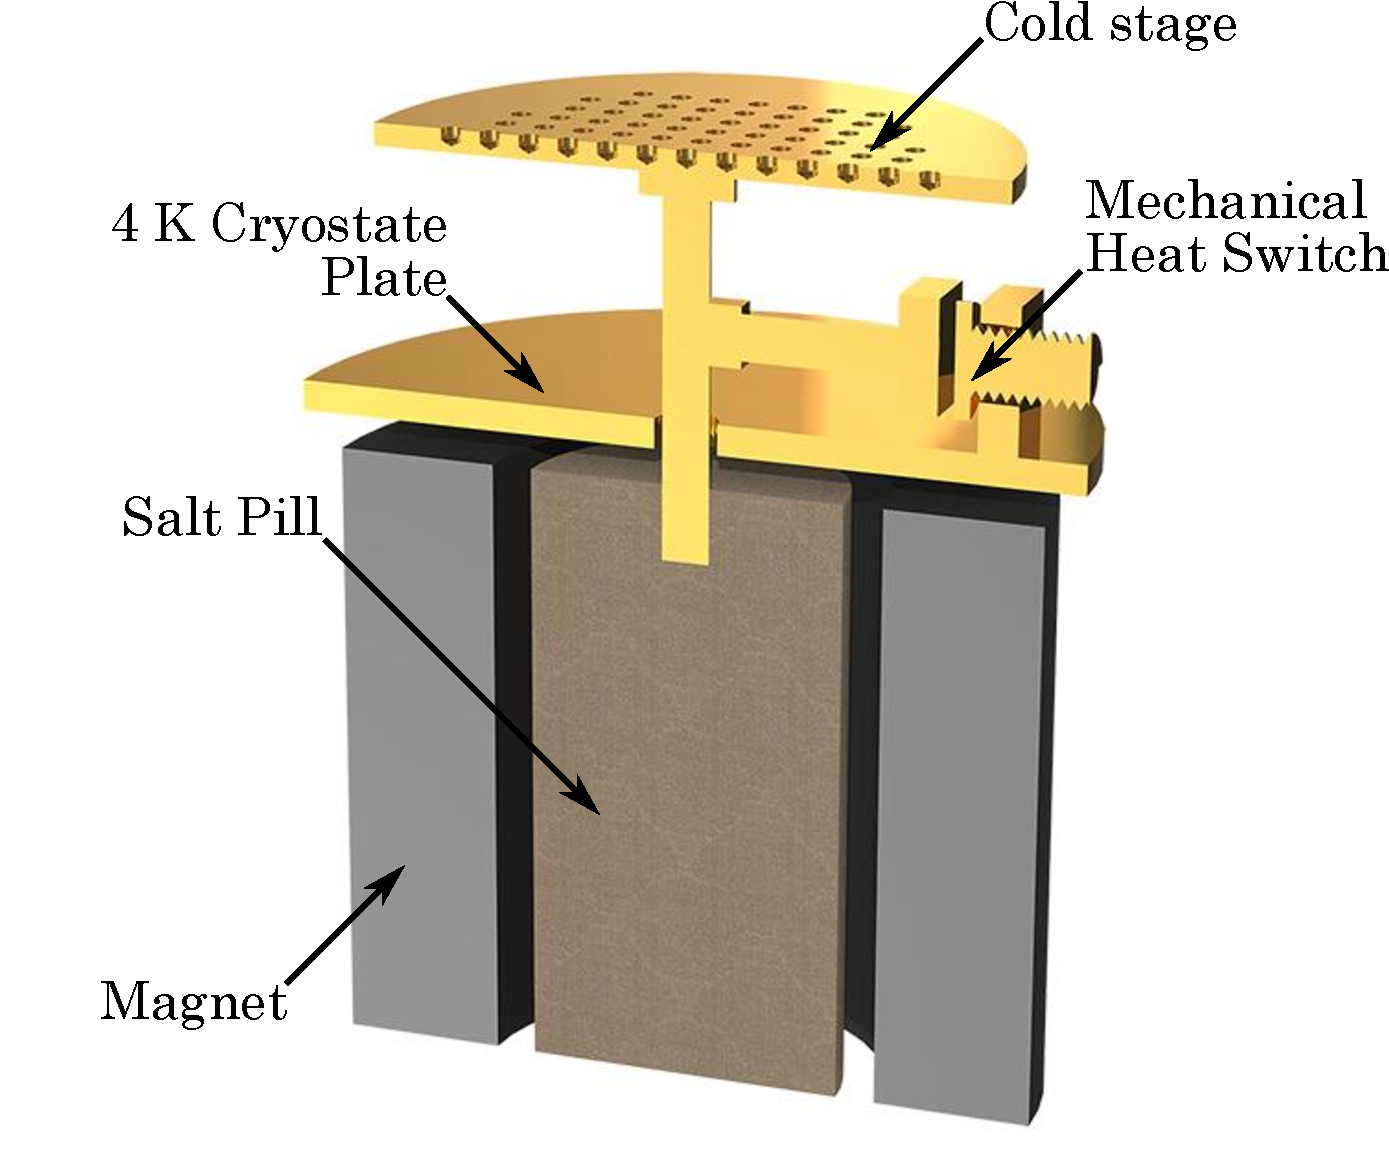
\includegraphics[width = 0.8\textwidth]{figures/ADR.pdf}
\caption[Artistic impression of a simple single-stage adiabatic demagnetisation refrigerator]{Artistic impression of a simple single-stage adiabatic demagnetisation refrigerator. The 4-Kelvin plate of the cryostat is cooled by either a liquid-helium reservoir or a mechanical cooler (not shown in either case).}
\label{fig:ADR}
\end{center}
\end{figure}
